% group articles by domain 
% for every article write a short summary of its relevant features
% and add an illustrative picture
% then criticize the presented solutions

\subsection{Multimodal Interfaces}

\subsubsection{Hardware Setups}

In order to obtain an immersive experience, there's a number of hardware
setups commonly available:

\begin{description}
	\item[Head-Mounted Display (HMD)] --
	  Head-mounting displays are glass-shaped devices, projecting a pair of stereo
	  transformed images to the user's retinas.
	  They normally feature a gyroscope or similar apparatus to measure head orientation and tilt.
	  There are two kinds of HMDs: in the former the images are projected in small opaque screens;
	  in the latter the projected surface is translucid, allowing blending of real and virtual worlds.
	  Translucid HMDs are best crafted for Augmented Reality (AR).
	  
		Using an HMD has the benefit of sticking to the user's head and detecting head orientation.
		On the other hand each HMD serves one single user and it has limited resolution.
		Additionally, most users report suffering from fatigue after long periods of
		usage \cite{VREDUC}.
		Opaque HMDs have the additional downside of users being unable to see the real world, 
		which can be confusing as noted by \cite{VANDERPOL}.
			
	\item[Cave Automatic Virtual Environment (CAVE)] --
	  A CAVE is an immersive virtual reality environment where projectors are directed to four,
	  five or all the six walls of a room-sized cube.
	  
		It shares the benefit of enclosing the user's viewing area with HMDs.
		Has a better resolution though.
		The downside is the small number of simultaneous users who can experience the CAVE at the same time.
	
	\item[Power Wall] --
	  A power wall is a large surface, usually planar, filled by an image.
	  The whole image projection is responsibility of a cluster of projectors set up in a wall.
	  Each projector renders part of the surface and the border between projections is ideally minimal.
	  Each projector is controlled by an independent computer.
	  
		Its size and resolution depend entirely on the setup, but normally a wall offers high resolution
		(depends on the number of projectors in the grid and each projector's resolution).
		Due to the large surface of the wall, several users may be served as once. Another benefit
		is users freedom of movement due to users not carrying wires \cite{INTTABLE}.
		The downside is users having to face the wall to experience the image entirely.
\end{description}

\begin{figure}[!ht]
	\centering
	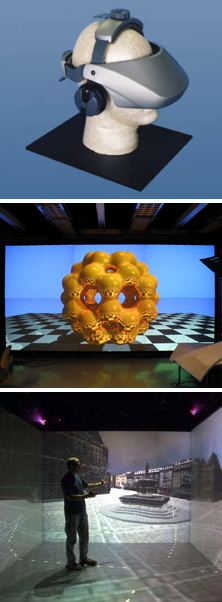
\includegraphics[width=12cm]{gfx/hmd-cluster-cave.png}
	\caption{HMD, Wall, CAVE}
	\label{FIG-HMD-CLUSTER-CAVE}
\end{figure}

Any of these setups is suitable for single user interaction.
In case of a reviewing session, in which at least two participants are required,
CAVE or Wall are better suited, since they alone offer a solution for a small group.

Using a Wall or CAVE presents other challenges: the computers responsible for
generating each projectors' images must be synchronized, its color parameters calibrated
and the viewport must be well cropped.
Several systems exist capable of delivering high performance 3D graphics and
offering the features mentioned above.
Based on scene graphs there are two well established solutions:
OpenSceneGraph\cite{SITE-OSG}
and
OpenSG\cite{SITE-OPENSG}.

\subsubsection{User Input}

Obtaining user input can be performed by an infinite combination of interfaces.
In Virtual Reality (VR) the most common solutions may feature a combination of:
\begin{description}
	\item[Image Processing] --
		A camera or a set of cameras continuously captures the environment and detects relevant
		features using vision algorithms.
		Subjects' position and orientation may then be determined using triangulation techniques.
	\item[Speech Recognition] --
		Users give specific verbal orders captured by a microphone, 
		which are interpreted by a speech recognition engine.
		The freedom of speech allowed by the engine depends on its quality and the purpose of
		the recognition -- spanning from simple commands to free formed sentences.
	\item[Motion Tracking] --
		This method is akin to image processing, but optimized for tracking subjects position
		and orientation.
		Small reflective markers are attached to each subject's relevant parts and infrared cameras
		are calibrated in order to read the markers and determine their position
		and orientation precisely.
		See Fig.\ref{FIG-MOTION-TRACKING}.
	\item[HMD's Rotation Data] --
		When a user is wearing an HMD device, its head rotation and tilt data can be captured,
		allowing the virtual world to act accordingly, e.g. rotating and tilting the VR world.
	\item[Tracked Artifacts for Direct Manipulation] --
		When motion tracking is available, users can manipulate artifacts and their positioning and
		orientation. This data can determine actions in the world, e.g. point at something, dragging, rotation.
	\item[Space Ball, Space Pilot, etc.] --
		These are special devices which allow 6 degrees or freedom (6DOF) manipulation.
		The user holds the device in his hands and the device's data can map several actions to
		the read axes.
		See Fig.\ref{FIG-SPACE-DEVICES}.
\end{description}

\begin{figure}[!ht]
	\centering
	\subfigure[
		Motion tracking example:
		the subject wears a suit with several markers distributed so that his skeleton
		relative orientations can be reasoned.
		An array of infrared cameras is rigged to the ceiling, reading marker positions.
	]{\label{FIG-MOTION-TRACKING}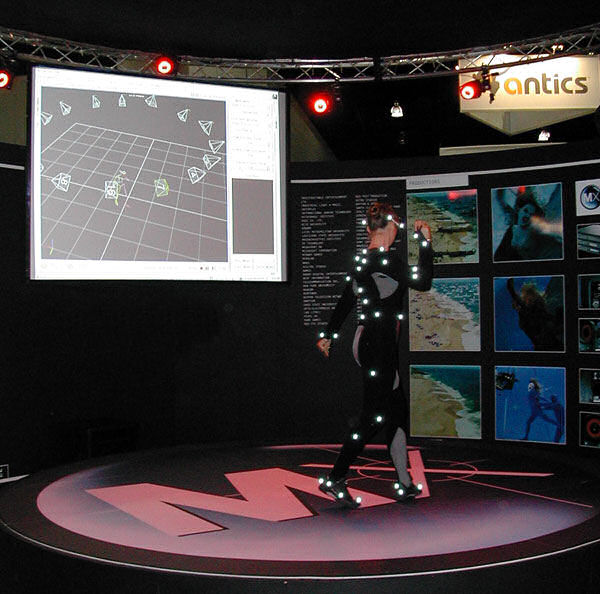
\includegraphics[width=5.5cm]{gfx/MotionCapture.jpg}}
	\subfigure[
		Two kinds of space balls and one space pilot.
	]{\label{FIG-SPACE-DEVICES}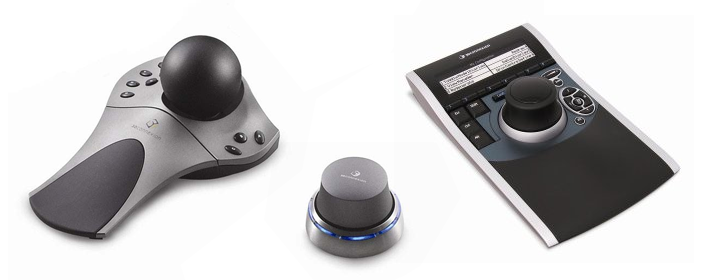
\includegraphics[width=6.5cm]{gfx/space-devices.png}}
	\caption{Interfaces}
\end{figure}

\subsubsection{Studies and Systems}

%Huot et al. \cite{TOW3D}.

% POST
Bistr�m et al. \cite{POST} present requirements for an efficient
post-WIMP\footnote{WIMP stands for Windows, Icons, Menus, Pointing \cite{WIMP}.} user interface,
focusing on navigation, selection and manipulation of objects.
WIMP interfaces can't cover all today's user needs. WIMP widgets are individually easy to
learn, but hard to aggregate. The discrete steps in dialog/menu interfaces divert the user
from the realtime working feel and denies the user from performing parallel actions.

Many studies have demonstrated 3D application development to be significantly more difficult
to implement than their 2D counterparts. Simple adaptation of 2D WIMP interfaces to three
dimensions does not provide a good solution to the problem. There's not one technique identified
as the best for this problem -- the solution must be based on the requirements of each application case.

Bistr�m et al. suggest an interface where both hands are used. The most precise work, such as manipulations,
is handled by the dominant hand. The non-dominant hand handles rough positioning or switches between
navigational modes.

Google Earth's \cite{SITE-EARTH} interface is identified and the following limitations found:
\begin{itemize}
	\item Only one object is in study (the planet Earth);
	\item The meta data layers have scarce interaction features;
	\item The view manipulation and moving of the planet is limited to one movement at a time.
\end{itemize}

A post-WIMP user interface is then devised for Google Earth. Two mice are given to the user.
The beginning screen presents all solar system planets and the user can pick a planet to examine.
Planet manipulation is similar to Google Earth's default view but no mouse pointer is available.
The dominant hand mouse controls the rotation of the object around X and Y axes if the primary mouse button is pushed. The non-dominant hands mouse controls the movement on the Z axis which is equal to
zooming if it is moved vertically if the primary mouse button is pushed.

The user must understand the use of the two mice and the functions of the mouse
buttons before he starts.
Managing  two 2D controls requires good manual skills and precision from both hands
and the ability to observe, process and control things is parallel,
which generally is not needed in desktop computing. 
Correcting of navigational errors is however easy as the natural reflex of rewinding the control
compensates the faulty action.

Application performance is expected to be better than in the original application
as different commands and actions can be given in parallel.
The 2D mouse controls produce continuous logarithmic output, an advantage
when comparing to using the equivalent discrete actions offered by keyboard or mouse pointed buttons.

\vspace{0.5cm}

% VREDUC
Kaufmann and Schmalstieg \cite{VREDUC} propose a collaborative Augmented Reality (AR)
system named Construct3D for teaching high school students 3D modeling.
It supports two users wearing see-through head-mounted displays with tracked heads and styluses
(see Fig. \ref{FIG-VREDUC} left).

Precise geometry construction is pointed out as difficult to accomplish in 3D space by direct
manipulation in 6 degrees of freedom due to tracking inaccuracies, lack of hand-eye coordination,
hand tremor and difficulties in precisely locating a 3D point presented with a fixed-focus
stereoscopic device.
This problem was solved by restricting the user's input to two dimensions and
providing grids and snapping functions to enable precision modeling.

Kaufmann and Schmalstieg give low importance to environment coordinates as indications of
position in space in a dynamic construction scenario.

\begin{figure}[!ht]
	\centering
	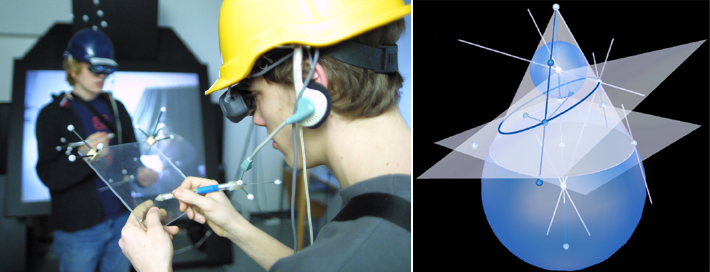
\includegraphics[width=10cm]{gfx/vreduc.png}
	\caption{Construct3D:
		user interface (left);
		proof that the intersection of plane and cone are either ellipse, hyperbola or parabola -- planes can be dynamically moved (right)}
	\label{FIG-VREDUC}
\end{figure}

\vspace{0.5cm}

% FREED
Wesche and Seidel \cite{FREED} present a sketching system named FreeDrawer.
It allows curve drawing and editing. The user wears a head-mounted display and handles a stylus
with the dominant hand with which the drawing is made. The remaining hand controls positioning
and orientation. The system's purpose is to allow conceptual design creation.
The system hides its internal complexity (B-spline curves and Catmull-Clark surfaces).
It estimates connectivity between curves by a threshold maximum distance.

\begin{figure}[!ht]
	\centering
	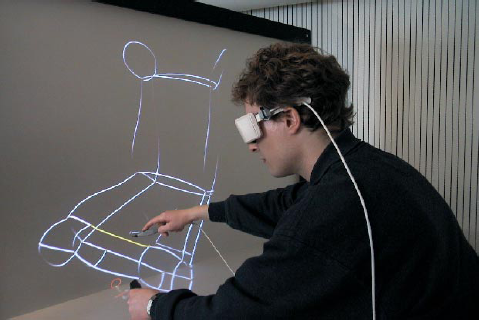
\includegraphics[width=6cm]{gfx/freed1.png}
	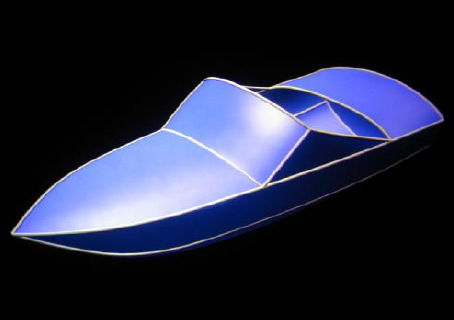
\includegraphics[width=6cm]{gfx/freed2.png}
	\caption{FreeDrawer:
		a user sketching a cushion (left);
		a boat modeled with the system (right)}
	\label{FIG-FREED}
\end{figure}

%\cite{INTTABLE}
%powerwall interaction problems, interaction table as solution

%\cite{TANINT}
%digital tape drawing and eraser pen to design 3d curves for automotive design

%\cite{GROSS}
%3D modeling on large displays: construction planes, tape drawing, 2 hand interaction

\vspace{0.5cm}

% WAND
Cao and Balakrishnan devise an input technique to serve large display interaction \cite{WAND}.
VisionWand is a plastic rod with colored ends, tracked by two low budget cameras.
The tracking results in a 3D ray. Since the rod has no electronics to support button clicking
or similar actions, a set of gestures was defined to allow user command input
(see Fig. \ref{FIG-VISIONWAND}).
VisionWand points out interesting functionality for the tracking data:
pointing with different ends of the wand invokes either manipulation or query actions,
while parallel posture activates a menu.
Distance from wand to screen serves as zooming factor where applicable.
In pie menus, wand orientation controls option selection.

\begin{figure}[!ht]
	\centering
	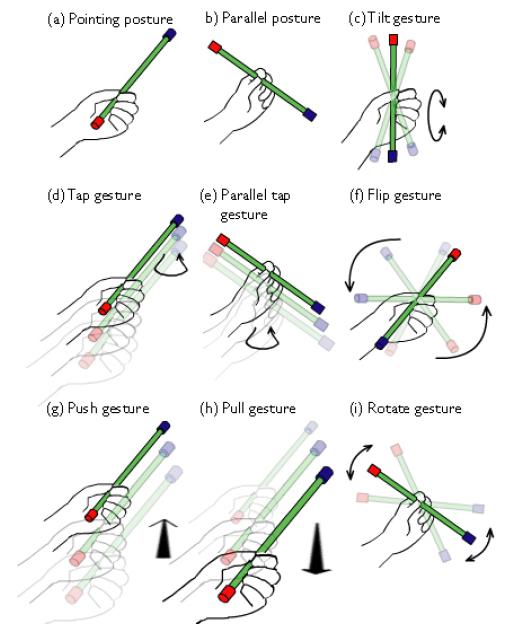
\includegraphics[width=4.5cm]{gfx/visionwand.png}
	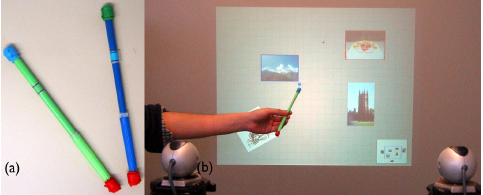
\includegraphics[width=7.5cm]{gfx/visionwand2.png}
	\caption{VisionWand: set of gestures(left); wands and hardware setup (right)}
	\label{FIG-VISIONWAND}
\end{figure}

%\cite{GESREC}
%hand tracking for gesture recognition. Forward HMMs and NNs tested.

\vspace{0.5cm}

% WBOARD
In informal group meetings or small lectures, a whiteboard is often used as the central
communication medium. Participants gather in front of the whiteboard and anyone
can scribble text or diagrams to share his or her thoughts.

Rekimoto \cite{WBOARD} presents a digital whiteboard where each participant is given
a palmtop computer. It works as a tool palette, remote commander, text entry box as
well as a temporary data buffer during whiteboard collaboration interaction.

Usual digital whiteboards suffer from the following limitations:
\begin{description}
	\item[Difficult text entry] --
		Current digital whiteboards have limited precision and tracking rate, making
		writing in it harder than on a conventional whiteboard. The resulting pen strokes
		and characters are often shaky and hard to read, not only for the computer (i.e. optical
		character recognition software) but also to humans. Even though computer recognizable characters are
		not strictly necessary, are far easier to move, copy, erase or search than unrecognized strokes.
		Recognized texts are also valuable for retrieving information from meeting logs.		
	\item[Large display renders current GUIs ineffective] --
		Many desktop sized applications features a menu bar at the top and toolbars at top/left of the
		window. This layout isn't suitable for large displays since it causes out-of-reach problems.
	\item[Whiteboard interactions become a bottleneck] --
		Most existing whiteboard applications are designed to be used by one user at a time.
		Single-threaded features such as pop-up or pull-down menus prohibit parallel activities
		among	collaborators.
\end{description}

\begin{figure}[!ht]
	\centering
	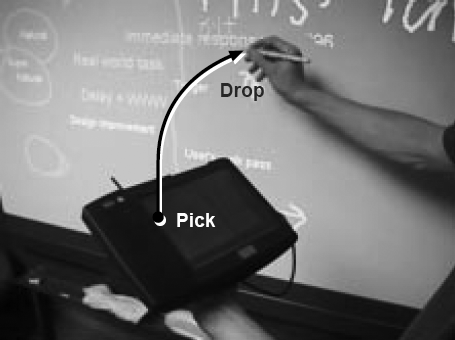
\includegraphics[width=6cm]{gfx/wboard.png}
	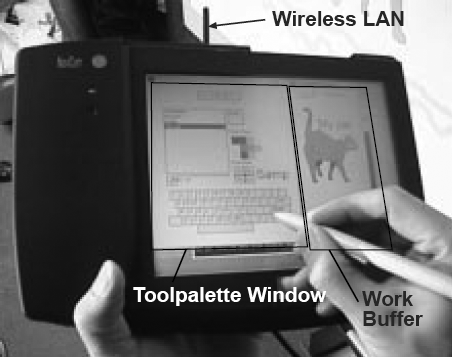
\includegraphics[width=6cm]{gfx/wboard2.png}
	\caption{Digital Whiteboard:
		Pick-and-drop interaction (left);
		Working areas for each participant's palmtop (right).}
	\label{FIG-WBOARD}
\end{figure}

Their solution involves each participant carrying a palmtop with a pen. The pen works both
with the palmtop and the digital whiteboard. A direct manipulation method called Pick-and-drop
(see Fig. \ref{FIG-WBOARD} left) was developed. It allows a user to pick an object in his
palmtop and dropping it in the whiteboard.  From an implementation point of view
data is transferred through the network, but from the user's perspective
this technique allows himto  pick up digital data as if it were a physical object.
Text entry is performed on the PDA and each user can use the method he favors (i.e.:
handwritten recognition, softkeyboard or simplified stroke input methods such as Unistroke
or Graffiti).
Instead of placing tool palettes or menu bars on the whiteboard, participants would have their own
tool palettes on a PDA.

The main window is a multi page tool panel. A user can flip to several tool palette
pages by selecting page tabs on top of the window.
The other window is a temporary work buffer. A user can store several data elements in this window
and paste them to the whiteboard using Pick-and-Drop operations. (see Fig. \ref{FIG-WBOARD} right).

Rekimoto concludes that putting many functions on the palmtops, users tend to concentrate too much
on their own palmtop devices, thus degrading mutual awareness among the participants.
Pick-and-Drop often worked better than drag-and-drop, particularly when user had to move objects
for a long distance. Drag-and-drop forces a user to keep the pen tip in contact with the board
during the entire operation, a restriction not suitable for large display surfaces.

%\subsubsection{Discussion}
%\TODO{Multimodal discussion}

\subsection{Sketching}
\subsubsection{Beautification}

% BEAUTY97
Igarashi and Hinckley present a 2D sketching system named Pegasus \cite{BEAUTY97}.
It receives user strokes and converts them, generating candidates by taking into
account restrictions for:
vertex connection, segment connection, parallelism, perpendicularity,
alignment, congruence, symmetry and interval equality.

The application presents the most relevant candidates to the user and highlights
the highest relevant one.
The user can either accept it or select another candidate by tapping on it as seen
in Fig. \ref{FIG-PEGASUS}.

\begin{figure}[!ht]
	\centering
	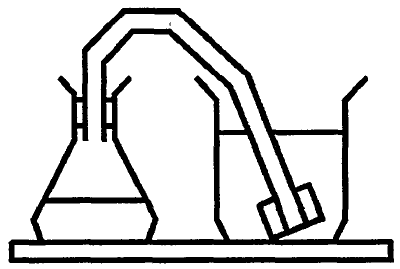
\includegraphics[width=5cm]{gfx/beauty97-1.png}
	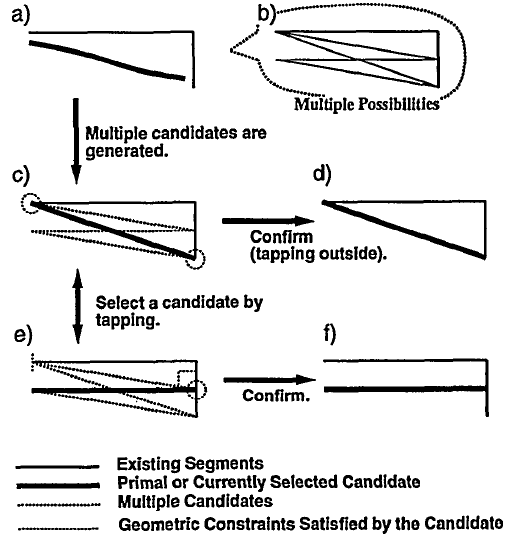
\includegraphics[width=5.5cm]{gfx/beauty97-2.png}
	\caption{Pegasus: A diagram drawn on Pegasus without using any editing commands such as rotation,
		copy or griding (left); interaction with multiple candidates (right).}
	\label{FIG-PEGASUS}
\end{figure}

\subsubsection{2D to 3D Reconstruction}

% DIGCLAY00
Digital Clay \cite{DIGCLAY00} allows a user to draw freely and tries to convert the drawing into a 3D model.
See input and 3D result in Fig.\ref{FIG-DIGCLAY}.

It uses two techniques to achieve that:

\begin{description}
	\item[The Huffman-Clowes algorithm], which identifies concave and convex vertices,
	requiring every line to connect to another line.
	The program additionally demands the object drawn to be solid;
	\item[The 3D coordinates are inferred] based on inherent rules that govern each type of drawing projection.
	i.e.: axes of isometric drawings have equal angles between them;
	perspective drawings show foreshortening of lines as we get closer to the viewer.
\end{description}

The downfalls of this method are the impossibility of describing occluded faces and
the limited editing capacities available once the conversion has been done.

\begin{figure}[!ht]
	\centering
	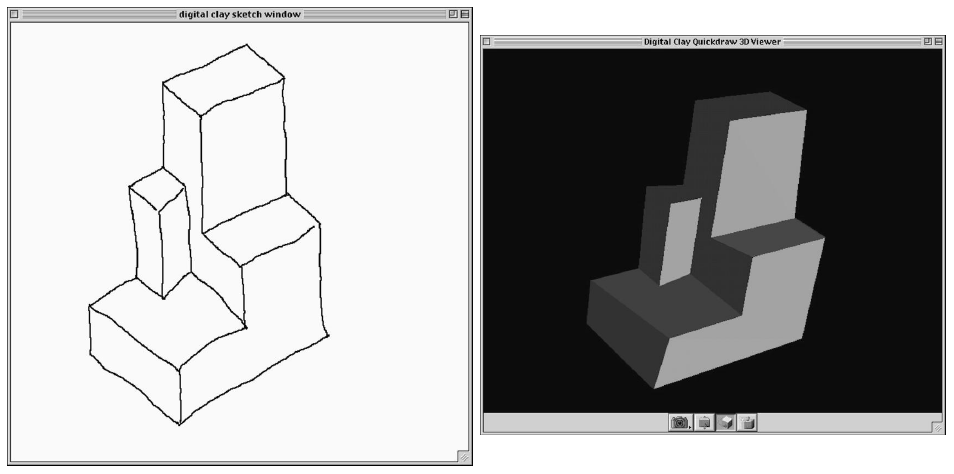
\includegraphics[width=11cm]{gfx/digclay00-1.png}
	\caption{Digital Clay: Raw sketch input and its 3D interpretation.}
	\label{FIG-DIGCLAY}
\end{figure}

\subsubsection{Suggestive Interfaces and Grammars}

% SMARTS01
Wenyin et al. created Smart Sketchpad \cite{SMARTSK01}.
Smart Sketchpad recognizes standard shapes (rectangles, triangles, ellipses, straight lines)
and compound shapes such as arrowheads.

The article describes the steps necessary for shape recognition:
\begin{enumerate}
	\item Input as a chain of points;
	\item Polygonalize to polyline and refine endpoints;
	\item Close near endpoints. If closed go to step 6;
	\item If line ends near another line end, join them and go to step 3;
	\item Classify line as one of: straight line, polyline or free form curve. Go to step 8;
	\item Close shape recognition; *
	\item Estimate the parameter of the closed shape;
	\item Test if shape can be combined with other shapes in the drawing. If so repeat step 8, else end.
\end{enumerate}

The $6^{th}$ step was tested with both rule-based systems, support vector machines and neural networks.
The most successfully approach was SVN, with 97,5\% success, closely followed by NN.

\vspace{0.5cm}

% FREEDOM01
Alvarado and Davis present a work towards an interface for mechanical designers named Assist \cite{FREEDOM01},
with the purpose of allowing them to sketch naturally and have the computer interpreting
their strokes into shapes like rods, hinges, polygons, etc.

The interpretation is a three stages procedure:

\begin{itemize}
	\item Match strokes to a series of templates;
	\item Rank interpretations with several heuristics about drawing style and mechanical engineering;
	\item Return the most consistent hypothesis.
\end{itemize}

Fig.\ref{FIG-FREEDOM01} illustrates the result.

The authors emphasize the difficulty they faced when replacing the original
human-made strokes by its computer interpretations.
Users prefer composing the whole drawing prior to computer interpretation replacement,
as opposed to a changeable estimation that refreshes at every added stroke.
Having the computer interpreting every stroke makes them feel they're losing control of the program. Even so, that was the path chosen by the authors because every extra stroke without giving feedback to the user increases the chance of misinterpretations.

Another relevant conclusion is that users expect symmetry to be kept regarding the interpreted
shapes, so it would be a good idea to detect and suggest alignment restrictions between shapes.

\begin{figure}[!ht]
	\centering
	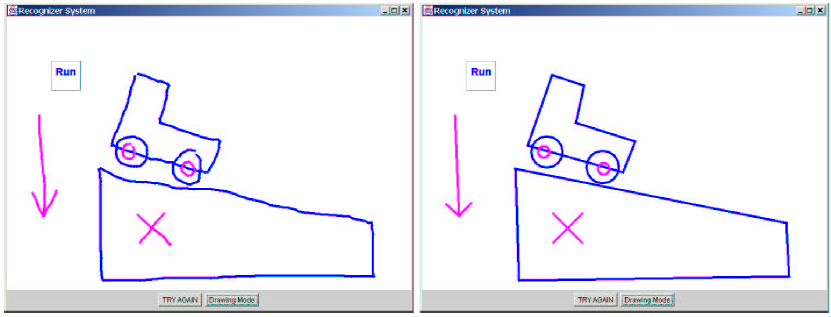
\includegraphics[width=11cm]{gfx/freedom01-1.png}
	\caption{Assist: A car on the hill. Drawn by the user (left), as interpreted and displayed (right).}
	\label{FIG-FREEDOM01}
\end{figure}

%\subsubsection{Discussion}
%\TODO{REVIEW THIS}
%Igarashi at al. present in \cite{BEAUTY97} a useful way of aiding the user.
%Most elements in architecture subsume to these constraints.
%Applying a technique of this kind gains more relevance in
%the 3D architecture problem because users will be modeling in 3D.
%Humans are more prone to drawing errors in a task like this,
%benefiting more from beautification algorithms.
%
%In \cite{SMARTSK01} a useful comparison between alternative implementations of their
%shape recognition algorithm is performed.
%Wenyin at al. conclude in their paper that Support Vector Machines are the faster implementation.
%The proposed algorithm itself is relatively simple and may be generalized to 3D shapes.
%
%The method proposed by Alvarado and Davis in \cite{FREEDOM01} works nicely but has applications
%only in 2D space.
%Additionally, users felt uneasy as the geometric shapes they drawn kept continuously being
%replaced by the computer program, making them feel having lost control of the application.
%
%Schweikardt and Gross \cite{DIGCLAY00} developed the only system discussed here that allows 3D drawing.
%Though its results are interesting, it shouldn't be used because it only allows describing part
%of geometry (the occluded geometry is undefined) and because it doesn't allow successive
%iterations to fill in the undefined geometry.

\subsection{Navigation}

% SMARTCAM05
In order to ensure users not ``getting lost'' in the virtual space,
Buchholz, Bohnet and D�llner \cite{SMARTCAM05}
propose a camera that is is both smart and physically-based.
It is smart in the sense that it is aware of confusing,
disorienting viewing situations, providing means to circumvent them.
It is physically based because it is supported by a physically based model of 3D motion
to ensure steady, continuous user movements.

In order to solve the disorientation problem, the camera must identify situations
when to intervene.
For that matter a metric, called orientation value, was created.
Each view is classified by counting its pixels, granting each one a different value:
landmarks are granted the highest values; terrain gets high values and sky gets low values.
A threshold can then be established and views below it are classified ``disoriented''.

When such an event takes place, smart navigation techniques restrict camera control.
The constraints posed to user control must be as comprehensible as possible.
Camera movement should also be time-coherent and physically sound.

The maintenance strategy solves critical situations such as (see Fig.\ref{FIG-SMARTCAM1}, left):

\begin{enumerate}[a)]
	\item The user rotates the flight direction and causes the camera to look too far beyond the terrain border.
		The rotation is accepted but outweighed by a slight rear movement away from the border.
	\item The user is flying forward beyond the terrain border.
		The maintenance strategy temporarily tilts down the view direction until a maximum angle is reached.
	\item If no more tilting is possible, the strategy rotates the flight direction parallel to the terrain
		to fly along the terrain border.
\end{enumerate}

\begin{figure}[!ht]
	\centering
	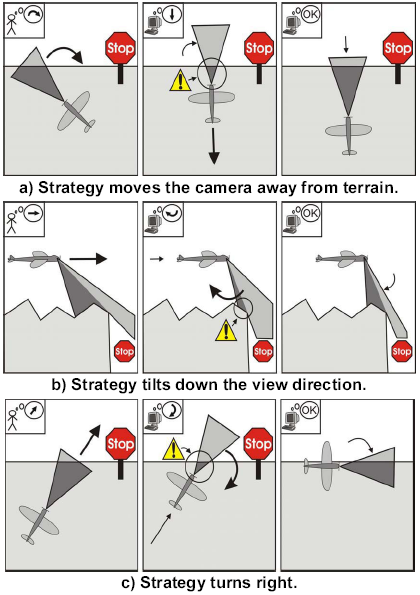
\includegraphics[height=7cm]{gfx/smartcam05-1.png}
	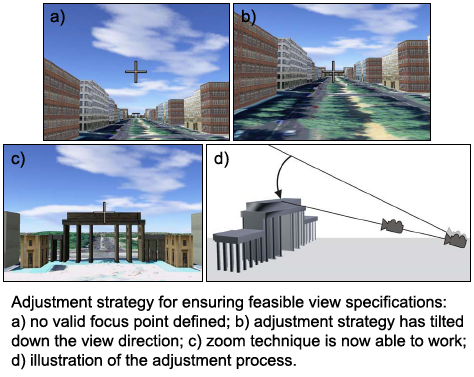
\includegraphics[height=5cm]{gfx/smartcam05-2.png}
	\caption{SPB Cam: Maintenance strategy for keeping high orientation values (left); Adjustment strategy for ensuring of feasible view specifications (right).}
	\label{FIG-SMARTCAM1}
\end{figure}

\vspace{0.5cm}

% WIM
LaViola et al. \cite{WIM} propose techniques for virtual environment navigation using walking, bending and turning.
The hardware setup is made of a 4 sided wall CAVE, one of the images being projected on the floor.
The user wears ``interaction slippers'' (adapted wireless trackballs assembled such that they
detect toe or heel joining) and a belt with a magnetic tracker mounted on the belt buckle.

The step World in Miniature (WIM) is a miniature version of the world that is projected on the ground,
under the user's feet in the virtual environment (see Fig. \ref{FIG-WIM}).
The user invokes the step WIM by joining his toes.
When in that state, walking translates user position in the scale emulating the movement in the projection,
functioning as an augmented road map. The translation is completed with another toe joining.
The system Distinguishes between moving in the WIM and finishing this state by tracking head direction:
if the head is 25� below the horizontal, the user is assumed to want to move to another place in the WIM,
otherwise step WIM mode is disabled.

\begin{figure}[!ht]
	\centering
	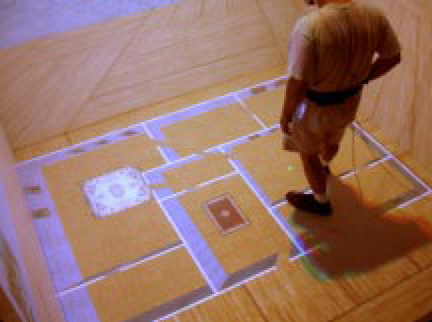
\includegraphics[height=5cm]{gfx/wim.png}
	\caption{Step WIM}
	\label{FIG-WIM}
\end{figure}

Step WIM scaling is enabled when user joins his heels. From that moment on until rejoining of the heels,
a change in the head angle with the horizontal changes step WIM scale.

Navigation can also be done by leaning in the direction one wants to move to. This is done by calculating
the vector between user's head and waist.

\vspace{0.5cm}

% NAVGE
Forlines et al. \cite{NAVGE} made a wrapper for Google Earth (GE) \cite{SITE-EARTH} with the purpose of
multiuser multidisplay interaction. Each machine runs a separate instance of GE. Besides the already
available layers of information GE supports, such as roads, hotel locations, country boundaries, etc.
its rendering pipeline can be extended through their KML file specification\footnote{http://earth.google.com/kml}. The wrapper has been tested between a touch table,
three wall displays and a tablet PC. The application is controlled through a combination of single-finger
mouse-like input.
On the table each member is represented by a small proxy camera whose position indicates rotation and
tilt relatively to the table's POV. It can be edited in the table or in the instance.
When a user changes position in the application, the wrapper polls GE his Point of View (POV), made up
of latitude, longitude, altitude, tilt, and azimuth. This data is sent over the network to the remaining
instances. 
Users can synchronize themselves with other members of the team or explore the map alone. This coupling
can be achieved by a simple tacking gesture to lock the camera proxy in-place or break the link.
Synchronized users focus on the same content even if at different locations. POV recalculation restricts
latitude and longitude change.
Different users may display different layers of information, as seen in Fig. \ref{FIG-NAVGE}.
Annotations are supported too. Each user can draw in his perspective and the annotations are geo-referenced
and sent to the remaining users. The annotation color of each user is coincident with his proxy color.

\begin{figure}[!ht]
	\centering
	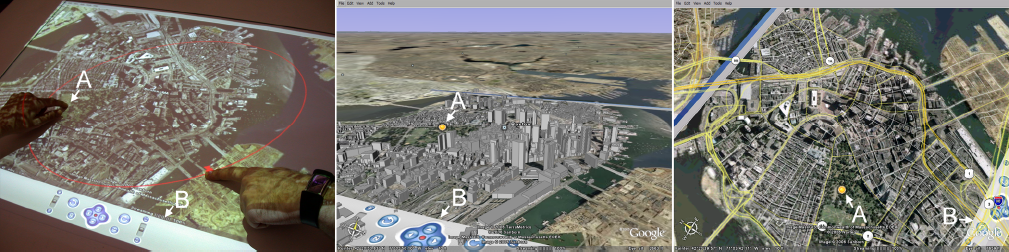
\includegraphics[width=12cm]{gfx/navge.png}
	\caption{Google Earth wrapper:
		two users manipulate member positions using the table. (left);
		two different instances with different layers displayed (center and right).
	}
	\label{FIG-NAVGE}
\end{figure}

\subsection{Knowledge Representation}

% LODCITY05
J�rgen D�llner and Henrik Buchholz \cite{LODCITY05} present a
solution for modeling buildings that feature continuous level of detail.

The authors propose the following levels of detail for a building (derived from
CityGML\footnote{CityGML is a common information model for the representation of 3D urban objects.
It defines the classes and relations for the most relevant topographic objects in cities
and regional models with respect to their geometrical, topological, semantical and appearance properties.
More info at: http://www.citygml.org}, see Fig.\ref{FIG-LODCITY}):

\begin{itemize}
	\item Simple block model
	\item Model with defined roof geometry
	\item Detailed indoor and outdoor building features
\end{itemize}

\begin{figure}[!ht]
	\centering
	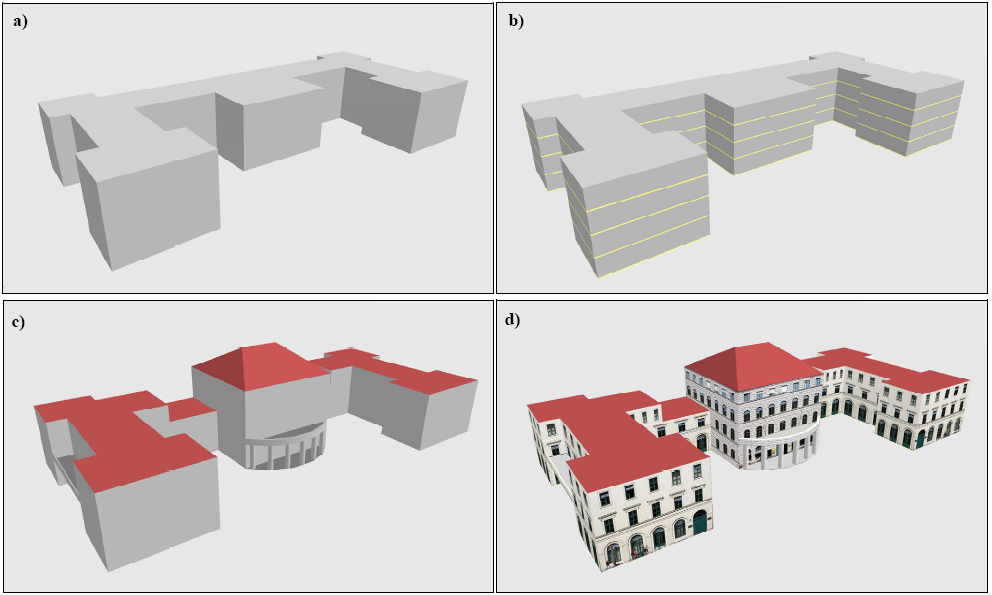
\includegraphics[width=11cm]{gfx/lodcity05-1.png}
	\caption{Continuous LOD: a) block model; b) building split into floors; c) geometry refinement; d) appearance refinement.}
	\label{FIG-LODCITY}
\end{figure}

A building is composed of a list of floor objects. A floor object refers to a floor prototype, which
contains the floor specification. This indirection allows a user to reuse floor prototypes in several
floors of the same building and allows rendering optimizations.

Each floor prototype is defined by its ground plan, which is one or more polygons that define the area
on which walls can be constructed. There can be inner loops in order to allow features like courtyards.
A ground plan supports thickness, useful for defining terraces.

On top of a ground plan one can place walls. A wall represents a vertical, planar polygon.
The default type of wall has no thickness, sufficient if a group of them form a closed surface
and can be only seen from the outside. Thick walls can also be added.
A wall can be lower or higher than its floor height, allowing balcony fronts and chimneys to be defined.

The higher ground plans can have roofs. The most common roof types are supported (hipped, gabled, tent,
mansard, pent, barrel) and a roof is described only by choosing the floor type and placing its
most relevant points (known as the roof skeleton).

Each floor prototype has a related floor decoration. A floor decoration is a collection of facade sections
and window sections. The former allows whole wall sections to be assigned a material while the latter
allows the definition of positioning and appearance of the floor's windows.

\subsection{Text Entry}

% PERLIN
Perlin proposes QuikWriting \cite{PERLIN}, a text entering technique using a style that allows
text to be introduced without stylus being lifted from the surface nor stylus stopping its movement.
This writing area is arranged in a 3x3 grid, numbered 1 through 9, arranged around a central
resting zone (5).
To form a character, the user drags the stylus from the central resting zone out to one of
the eight outer zones (1,2,3,4,6,7,8,9), then optionally to a second outer zone and finally
back to the resting zone.
Gestures are chosen so that frequent characters can be entered very rapidly.
Certain gestures shift to alternate character sets.

\begin{figure}[!ht]
	\centering
	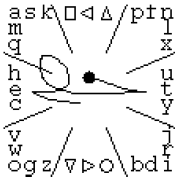
\includegraphics[width=3cm]{gfx/perlin.png}
	\caption{QuikWriting: method for writing the word ``the''}
	\label{FIG-PERLIN}
\end{figure}

\vspace{0.5cm}

% GRAF
Erdem et al. \cite{GRAF} adapted the Graffiti\texttrademark alphabet popular in palmtop devices for usage
in a wall with laser as pointing device.
The alphabet was simplified (see Fig. \ref{FIG-GRAF}) in order to allow continuous character input
and increase recognition accuracy. Each character is done with a single stroke.
The alphabet is easily learned due to its resemblance with the roman alphabet.

\begin{figure}[!ht]
	\centering
	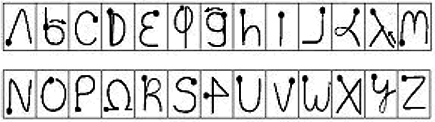
\includegraphics[width=6cm]{gfx/graf.png}
	\caption{Modified Graffiti alphabet. Dots mark the beginning of the stroke.}
	\label{FIG-GRAF}
\end{figure}


\vspace{0.5cm}

% GLYPH
Poirier \cite{GLYPH} isolated 6 simple shape primitives and drawn an alphabet made only with them
(see Fig. \ref{FIG-GLYPH}). Each letter has at most 3 primitives.
During experiments users improved their performance (12 characters per minute in first
session to 25 cpm in fifth session).

\begin{figure}[!ht]
	\centering
	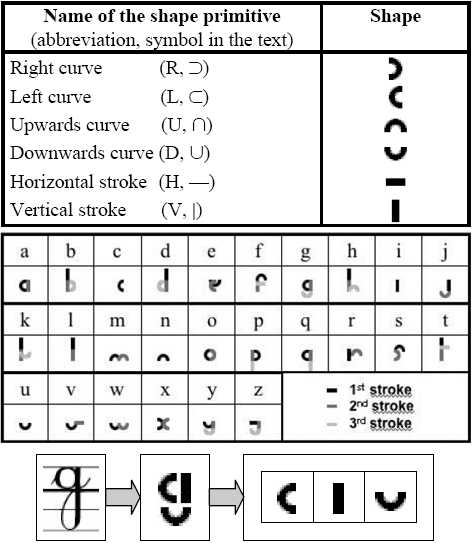
\includegraphics[width=8cm]{gfx/glyph.png}
	\caption{Glyph:
		the 6 shape primitives (top);
		alphabet composed of primitives (middle);
		the letter g decomposed (bottom)}
	\label{FIG-GLYPH}
\end{figure}

%\cite{CROSSY}
%It introduces a drawing application using goal crossing as a way to selecting actions.
%It proves to be flexible and allows a combination of goals to be learned by users and
%improve their performance with the interface.
%It is useful when WIMP isn't possible (such as this case due to pen/wand usage)
%
%\cite{JOYCOMP}